\documentclass[11pt]{report}
\usepackage[utf8]{inputenc}	% Para caracteres en español
\usepackage{amsmath,amsthm,amsfonts,amssymb,amscd}
\usepackage{multirow,booktabs}
\usepackage[table]{xcolor}
\usepackage{fullpage}
\usepackage{lastpage}
\usepackage{enumitem}
\usepackage{fancyhdr}
\usepackage{mathrsfs}
\usepackage{wrapfig}
\usepackage{setspace}
\usepackage{hyperref}
\usepackage{calc}
\usepackage{multicol}
\usepackage{cancel}
\usepackage[retainorgcmds]{IEEEtrantools}
\usepackage[margin=3cm]{geometry}
\usepackage{amsmath}
\newlength{\tabcont}
\setlength{\parindent}{0.0in}
\setlength{\parskip}{0.05in}
\usepackage{empheq}
\usepackage{framed}
\usepackage[most]{tcolorbox}
\usepackage{xcolor}
\colorlet{shadecolor}{orange!15}
\parindent 0in
\parskip 12pt
\geometry{margin=1in, headsep=0.25in}
\theoremstyle{definition}
\usepackage{pdfpages}
\newtheorem{defn}{Definition}
\newtheorem{reg}{Rule}
\newtheorem{exer}{Exercise}
\newtheorem{note}{Note}
\usepackage{fancyhdr}\usepackage{xcolor}\usepackage{amsmath}\usepackage{amssymb}\pagestyle{fancy}\rhead{}
\newtheorem{theorem}{Theorem}[subsection]
\theoremstyle{definition}
\newtheorem{definition}[theorem]{Definiton}
\newtheorem{example}[theorem]{Example}
\newtheorem{corollary}[theorem]{Corollary}
\newtheorem{lemma}[theorem]{Lemma}
\title{Chapter 9 Review Notes}
\begin{document}
\thispagestyle{empty}
{\LARGE \bf CHE 260 Lecture Notes}\\
{\large Hei Shing Cheung}\\
Thermodynamics and Heat Transfer, Fall 2025 \hfill CHE260\\
\\
The up-to-date version of this document can be found at \url{https://github.com/HaysonC/skulenotes}\\

\begin{center}
    \textit{``If there is one word that describes this class it would be \textbf{energy}.''}
\end{center}
\chapter{Thermodynamics}

\section{Systems and Properties in Thermodynamics}
\begin{definition}[Energy]
    You should have learned that energy is the ability to do work.
\end{definition}


\begin{definition}[Work]
    You also learned that work is the transfer of energy.
\end{definition}

We have a problem. The above two definitions are in terms of each other. This touches on the theory of fundamental concepts:

\paragraph{Fundamental Concepts} For example, the following are fundamental concepts in physics:
\begin{itemize}
    \item Time
    \item \textbf{Mass} Interestingly, we don't measure mass directly; instead, we measure weight, which is the force exerted by gravity on an object, and from that we deduce mass.
    \item Space
\end{itemize}
In this course, we are going to explore two:
\begin{itemize}
    \item \textbf{Energy} Energy is pretty familiar to us. 
    \item \textbf{Entropy} Entropy is what gives students the most trouble; you can't show someone a picture of entropy, it is abstract.
\end{itemize}

These fundamental concepts are in arbitrary units and form the foundation `axioms' in science.

\subsection{Energy}
\paragraph{Energy} An understanding of energy is its ability to \textbf{lift weights}. This is a way we could test if there is energy.
\begin{example}[Potential Energy]
    A 1 kg mass lifted 1 meter has a potential energy of about 10 J. Imagine that it is attached to a balance, with a small mass on the other side, then, it is able to lift that weight.
\end{example}

\begin{example}[Kinetic Energy]
    Given a flying ball that hits a lever with a mass rested on it, given the appropriate angle, the ball can transfer its kinetic energy to the mass, causing it to lift.
\end{example}

\begin{example}[Heat]
    Given a gas in a container, if we heat the gas, it expands and lifts objects on top of it.
\end{example}
\begin{shaded}
\begin{example}[Newcomen Engine]
    The above example is actually a simplified representation of how the Newcomen engine operates. In the Newcomen engine, steam is used to create a vacuum that lifts a piston, demonstrating the conversion of thermal energy into mechanical work.
\end{example}
\end{shaded}
\begin{figure}[h!]
    \centering
    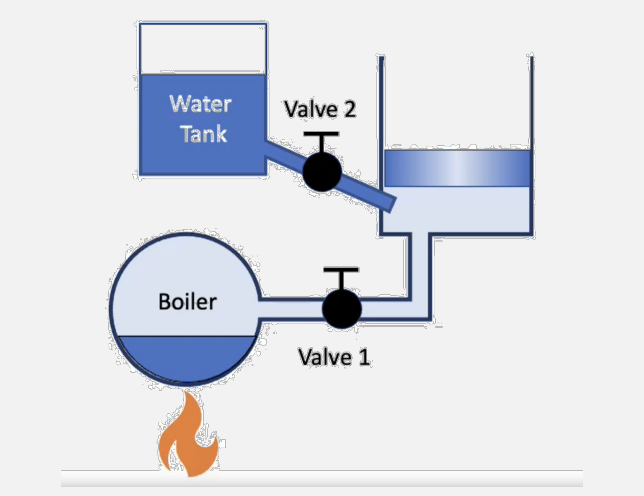
\includegraphics[width=0.5\textwidth]{newcomen_engine.png}
    \caption{A Newcomen Engine}
\end{figure}
When Valve 1 opens, steam fills the chamber and lifts up the piston. When Valve 2 opens (with valve 1 closes),
water gets sprayed, evaporates, and condenses, causing the piston to lower.

However, the Newcomen engine is not the most efficient steam engine, most heat is lost in the heating and cooling process. Solution? A external condenser was added to improve efficiency by cooling the steam and creating a vacuum, allowing the piston to be pulled down more effectively. This is the \textbf{Watt Engine}.

\paragraph{Steam Cycle} The steam cycle is a thermodynamic cycle that converts heat energy into mechanical work. It consists of four main processes: 
\begin{enumerate}
    \item \textbf{Heating} - The working fluid (steam) is heated in the boiler, converting water into steam and increasing its energy.
    \item \textbf{Expansion} - The high-pressure steam expands in the piston, doing work on the piston and converting thermal energy into mechanical work.
    \item \textbf{Cooling} - The steam is cooled in the condenser, releasing heat to the surroundings and condensing back into water.
    \item \textbf{Compression} - The water is pumped back into the boiler, completing the cycle.
\end{enumerate}

\begin{figure}[h!]
    \centering
    \begin{tikzpicture}
        \node (boiler) [rectangle, draw] {1. Boiler};
        \node (turbine) [rectangle, draw, right=of boiler] {2. Turbine};
        \node (condenser) [rectangle, draw, below=of turbine] {3. Condenser};
        \node (pump) [rectangle, draw, below=of boiler] {4. Pump};

        \draw[->] (boiler) -- (turbine);
        \draw[->] (turbine) -- (condenser);
        \draw[->] (condenser) -- (pump);
        \draw[->] (pump) -- (boiler);
    \end{tikzpicture}
    \caption{Steam Cycle Diagram}
\end{figure}

\begin{definition}[Heat Engine]
    A heat engine is a device that converts thermal energy into mechanical work. It operates by taking in heat from a high-temperature source, performing work using that heat, and then releasing some waste heat to a low-temperature sink. The steam engine is a classical instance of a heat engine.
\end{definition}
\begin{figure}[h!]
    \centering
    \begin{tikzpicture}
        \node (Engine) [circle, draw] {Heat Engine};
        \node (Source) [rectangle, draw, left=of Engine] {High-Temp Source ($Q_H$)};
        \node (Sink) [rectangle, draw, right=of Engine] {Low-Temp Sink ($Q_C$)};
        \draw[->] (Source) -- (Engine);
        \draw[->] (Engine) -- (Sink);  

        \node (Work) [rectangle, draw, below=of Engine] {Work Output ($W$)};
        \draw[->] (Engine) -- (Work);
    \end{tikzpicture}
    \caption{A Heat Engine}
\end{figure}

\paragraph{Efficiency of a Heat Engine} The efficiency of a heat engine is defined as the ratio of the work output to the heat input:

\begin{equation}
    \eta = \frac{W}{Q_H}
\end{equation}

Obviously, the best engine is when $\eta$ is maximized ($W$ is maximized, and $Q_H$ is minimized). For example, a Newcomen engine has a low efficiency ($\eta \approx 0.34\%$), while a classic watt engine has a higher efficiency ($\eta \approx 4\%$). The modern powerplant is optimized such that it has $\eta \approx 30\%$.

This begs the question, can we create a heat engine with 100\% efficiency (i.e., $Q_C = 0$)? The answer is no, due to the second law of thermodynamics [Sadi Carnot (1830)]. For now, consider the wasted energy $Q_c$. 

\paragraph{Irreversibility and Spontaneity} The process of losing heat is spontaneous and irreversible. Once heat is lost to the cooler surroundings, it cannot be completely recovered and converted back into work, however, the process of bringing heat from a cooler body to a hotter body is non-spontaneous and requires external work (e.g., a refrigerator). These give rise to the concept of irreversibility in thermodynamic processes, from the laws of thermodynamics.

The first law of thermodynamics is simple and easy to understand:
\begin{definition}[First Law of Thermodynamics]
    The first law of thermodynamics states that energy cannot be created or destroyed, only transformed from one form to another. In the context of a heat engine, this means that the work output ($W$) is equal to the heat input ($Q_H$) minus the heat rejected ($Q_C$):
    \begin{equation}
        W = Q_H - Q_C
    \end{equation}
\end{definition}
The second law formalizes the concept of the directionality of thermodynamic processes, stating that heat cannot spontaneously flow from a colder body to a hotter body. This law introduces the idea of entropy, a measure of the disorder or randomness in a system, which tends to increase over time in isolated systems.

\begin{definition}[Second Law of Thermodynamics]
    The second law of thermodynamics states that the total entropy of an isolated system can never decrease over time. We consdier entropy as:
    \begin{equation}
        S = \frac{Q}{T}
    \end{equation}
    In the above example, we can see that entropy increases as heat is transferred from the hot reservoir to the cold reservoir:

    $$
        \Delta S = S_{\text{final}} - S_{\text{initial}} = \frac{Q_C}{T_C} - \frac{Q_H}{T_H} > 0
    $$

    Since $Q_C = Q_H$ in a closed system and $T_H > T_C$, we have $\Delta S > 0$.
\end{definition}

\subsection{Modeling Ideal Gas}
\begin{definition}[Ideal Gas]
    We consider ideal gas conditions as those where the gas particles do not interact with each other except during elastic collisions, and the volume of the gas particles themselves is negligible compared to the volume of the container. In this course, we consider 1 atm as the threshold for ideal gas behavior. Of course, ideal gas obey the ideal gas law:
    \begin{equation}
        PV = nRT
    \end{equation}
\end{definition}

\subsection{Systems and States}
\begin{definition}[System]
    Any piece of matter or a region of space.
\end{definition}

\begin{definition}[Boundary]
    The boundary is the surface that separates the system from its surroundings. It can be real or imaginary, fixed or movable, and can allow or prevent the transfer of mass and energy.
\end{definition}

\textbf{Types of Systems} There are three main types of systems: closed, open, and isolated. Defined as the following:
\begin{definition}[Closed System/Control Mass]
    A closed system is one where mass cannot cross the boundary, but energy can. An example of a closed system is a sealed container of liquid, or a bag of gas, where we can do work on it.
\end{definition}
\begin{definition}[Open System/Control Volume]
    An open system is one where both mass and energy can cross the boundary. An example of an open system is a flowing pipe, or a car engine, where mass (water, air) and energy (heat, work) can enter and leave the system.
\end{definition}
\begin{definition}[Isolated System]
    An isolated system is one where neither mass nor energy can cross the boundary. An example of an isolated system is a thermos bottle that is perfectly insulated from its surroundings.
\end{definition}
\begin{definition}[Property]
    A property is any attribute of a system that can be measured without knowing the history of the system. \\
    (Example) Position, Temperature, Mass, Energy \\
    (Non-example) Work, Transfer of energy (heat), Mass outside the system (denote $\delta m$)
    \begin{equation}
        W = \int dW \quad (\text{depends on path})
    \end{equation}
    Hence, to remind ourselves, we denote infinitesimal work as $\delta W$ instead of $dW$. Then, we can compute the work done on a system as:
    \begin{equation}
        \delta W = \int_C F \, dx 
    \end{equation}
\end{definition}

\paragraph{Intensive and Extensive Properties} Properties can be classified into two categories: intensive and extensive.
\begin{definition}[Extensive Property]
    An extensive property is one that depends on the size or extent of the system. \\
    (Example) Mass, Volume, Energy
\end{definition}    
\begin{definition}[Intensive Property]
    An intensive property is one that does not depend on the size or extent of the system. \\ 
    (Example) Temperature, Pressure, Density 

    We can convert any extensive property to an intensive property by dividing it by mass or volume. For example, specific volume $v$ or specific energy $u$:
    $$
        v = \frac{V}{m}, \quad u = \frac{U}{m}
    $$
\end{definition}

\begin{definition}[State]
    The state of a system is defined by its properties at a specific moment in time. A state is a condition of the system that can be described by a set of properties. For example, the state of an ideal gas can be described by its pressure, volume, and temperature.
    
\end{definition}

\begin{definition}[Steady State]
    A system is in steady state if its properties do not change with time. In other words, the system is in a state of equilibrium, and there are no net changes in mass or energy within the system. \\
    (Example) An overflowing bucket of water, in which case the system is unchanging but interacting with its surroundings.
\end{definition}

\begin{definition}[Equilibrium]
    An \textbf{ISOLATED} system is in equilibrium if its properties are uniform throughout the system and do not change with time (constant). \\
    (Example) A gas in a closed container that has been left undisturbed for a long time.
\end{definition}
\begin{example}
    Consider a gas in a cylinder with a movable piston. If the piston is held in place, the gas is in a steady state, as its properties (pressure, volume, temperature) do not change with time. However, if the piston is allowed to move, the gas will expand or compress, and its properties will change with time, indicating that it is not in a steady state. 
\end{example}
\begin{definition}[Process]
    A process is a transformation from one state to another. A process can be described by the path taken by the system in the property space. For example, a gas can undergo a process of compression or expansion, which changes its pressure, volume, and temperature.
\end{definition}
\chapter{Heat Transfer}

\end{document}
